\section{Wie uns Google beeinflusst}\label{sec:wie-uns-google-beeinflusst}

\subsection{Der Einfluss von Google}\label{subsec:der-einfluss-von-google}
Mit einem Marktanteil von über 90 Prozent in Deutschland, im mobilen Sektor sogar über 96 Prozent, erfreut sich die Google Suchmaschine in den letzten Jahren immer größerer Beliebtheit.
Während das Rennen der Suchmaschinen vor etwa 20 Jahren noch ein \("\)bunte Mischung\("\) war, hat Google heute nahezu ein Monopol in diesem Bereich geschaffen.
Auch weltweit ist Google, wenn auch nicht so eindeutig wie das in Deutschland der Fall ist, mit Abstand auf Platz eins der beliebtesten Suchmaschinen.
Jeder von uns \("\)googelt\("\)\autocite{DUD22}, wie es die Suchmaschine schon in den deutschen Duden geschafft hat, im Schnitt dreimal am Tag.\autocite{DOL22}\\
Wenn man diese Zahlen hört, dürfte schon klar sein, dass Google unser Verhalten als Nutzer im Web maßgeblich beeinflusst hat.
Wie genau Google uns beeinflusst hat oder vielleicht noch beeinflussen wird, wird im Folgenden analysiert.

\subsection{Veränderung des Benutzerverhaltens mehrerer Generationen}\label{subsec:veränderung-des-benutzerverhaltens-mehrerer-generationen}
Modernisierung des Webs - das Google-Ranking bestimmt, ob und auf welchem Platz eine Webseite dem Nutzer bei einer Suchanfrage vorgeschlagen wird.
Um in diesem Ranking möglichst gut platziert zu werden, sollte man bestimmte Voraussetzungen erfüllen, so sei es beispielsweise wichtig die Webseite gut an die Ansicht auf Mobilen Geräten anzupassen.\autocite{BUI22}
Wie eine Statistik von statcounter zeigt, übertraf die Internetnutzung auf mobilen Geräten 2016 erstmals die Nutzung von einem Desktop aus mit einem ständigen Wachstum der mobilen Nutzung seit 2009.\autocite{STA16}
Nicht zuletzt dürfte dazu wohl auch die immer besser werdende Benutzerfreundlichkeit von Webseiten auf mobilen Geräten beigetragen haben.
Und weil Seiten mit einer guten Anpassung auf mobile Geräte von Google höher gerankt werden, ist es wohl kein Wunder, dass wir unsere mobilen Geräte auch für das surfen im Netz immer mehr benutzen können.
Auch in Zukunft, wenn der Trend weiter in Richtung mobile Geräte, wie eventuell auch SmartWatches oder Sprachsteuerung geht,
wird Google wohl signifikant mitbestimmen, inwieweit das World Wide Web zugänglich für neue Technologien wird.\\

Informationsbeschaffung - Informationsquellen, die Quellen, aus denen wir unser Individualwissen nehmen,
veränderten und vermischten sich in der Geschichte immer wieder aufs Neue.
Von reiner mündlicher Überlieferung über Buchdruck und Radio bis zum Fernsehen.
Doch wohl kaum gab es zuvor eine Quelle mit der man so schnell Informationen in vergleichbaren Mengen und aus vergleichbar vielen Quellen beschaffen konnte wie mit dem Internet.
Einem Bericht der \("\)mednic\("\) zufolge gaben 82 Prozent der Befragten 2020 an sich über Covid-19 im Internet zu informieren.\autocite{RKW20}
Ob über Nachrichtenseiten, Social Media oder Podcasts und egal über welches Thema,
Google und Co liefern uns Informationen und vor allem in jüngeren Generationen werden Suchmaschinen eine immer beliebtere Informationsquelle.\\

Konnektivität der Google Dienste - ob die Google Suchmaschine, Gmail, YouTube, Maps oder den Google Play Store,
die meisten von uns nutzen nicht nur eines der zahlreichen Google Produkte und Dienste.
In der Gmail-App kann man ganz einfach mithilfe von Google Drive auch größere Dateien anhängen und in der Google Suchmaschine kann man ganz einfach seinen YouTube und Gmail Account einbinden, alles mit Hilfe des Google Kontos.
Und das sind nur ein paar Beispiele, wie man verschiedenste Google Dienste vergleichsweise einfach miteinander verbinden kann.
\begin{figure}[ht]
    \centering
    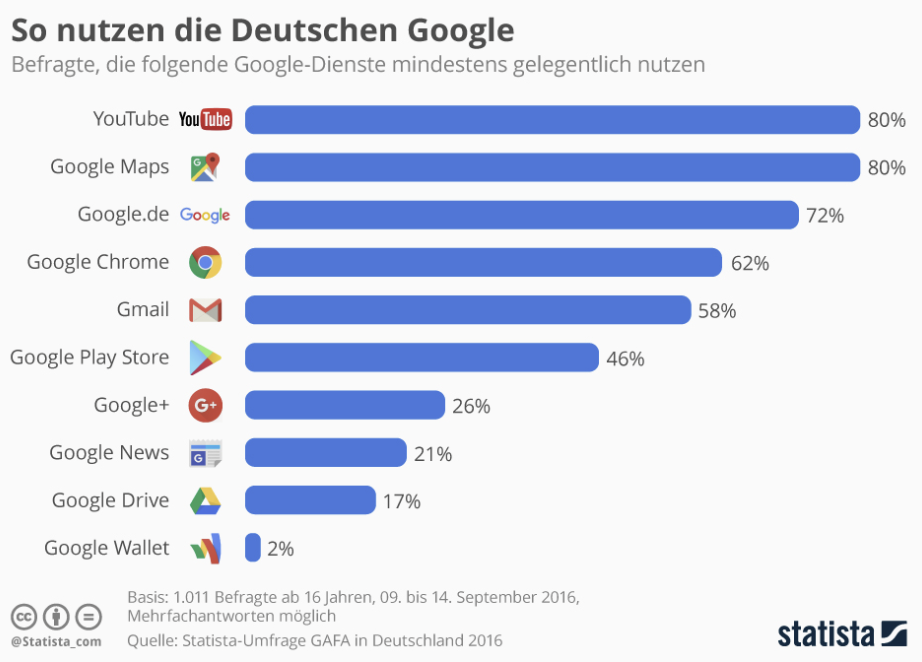
\includegraphics[width=100mm]{images/statistic_googleServices}
    \caption{Statistik Nutzung der Google Dienste in Deutschland}
    \label{fig:statisticGoogleServices}
\end{figure}  %https://de.statista.com/infografik/6020/nutzung-von-google-diensten-in-deutschland/
Wie in der Statistik zu sehen ist, nutzen bereits heute 80 Prozent der Menschen in Deutschland Google Maps und YouTube, dicht gefolgt von der Google Suchmaschine mit 72 Prozent.
Auch die restlichen Google Services sind in Deutschland gut vertreten und das wohl nicht zuletzt auch,
weil Google es uns in den letzten Jahren immer einfacher gemacht hat die verschiedenen Dienste miteinander zu verbinden.
Erst 2019 wurde Google+, was immerhin 26 Prozent der Deutschen nutzten, eingestellt.
Bei dem Google Dienst, der gerade einmal knapp 8 Jahre am Markt war, handelte es sich um ein soziales Netzwerk,
das \("\)mehrere Google-Werkzeuge [\ldots] in einem einzigen sozialen Netzwerk von Google\("\)\autocite{JEC21} vereinen sollte.\autocite{JEC21}
Und, auch wenn dieses Projekt gescheitert ist, sieht man daran, wie Google immer wieder versucht seine Dienste noch besser miteinander zu vernetzen.
Schon heute haben sich die Google features wie wohl kaum eines anderen Anbieter in unseren Alltag integriert,
und so wird Google wohl auch in Zukunft, wenn es vielleicht noch weitere Google Dienste geben wird, durch gute Konnektivität und eine dadurch verbesserte User Experience überzeugen.\\

UX und Einfachheit - Eine schlichte, meist weiße Webseite mit einer Suchbar in der Mitte und einem kleinen Bild darüber,
in den Grundzügen sieht die Landingpage der Google Suchmaschine schon seit es sie gibt so aus.
Mit kleinen der Zeit angepassten Modernisierungen selbstverständlich.
Die Nutzung der Google Suchmaschine könnte wohl kaum einfacher und selbsterklärender sein.
Usability beschreibt die Nutzbarkeit oder auch Gebrauchstauglichkeit eines Produktes und ist ein wesentlicher Bestandteil der UX (=User Experience),
die wiederum beschreibt wie gut die Erfahrung ist, die ein User mit dem Produkt im Durchschnitt macht, also wie einfach und komfortable ein Produkt für der User oder Anwender nutzbar ist.\autocite{Maulhardt4}
Durch die einfache und selbsterklärende Nutzung weißt Google eine ziemlich hohe Usability vor und nicht nur das,
die Usability ist auch ein wesentlicher Bestandteil des Rankings von Google, so gibt uns Google bevorzugt Ergebnisse aus, bei denen die Usability auch vergleichsmäßig hoch ist,
was ein weiterer Grund ist warum viele die Suchergebnisse von Google sehr schätzen und wohl auch in Zukunft noch schätzen werden.\autocite{LIC15}\\

Accessibility der Information - Das Ziel, das die Google Suchmaschine von Anfang an verfolgt hat,
ist es Informationen für Menschen erreichbar zu machen und die Benutzer sind es gewohnt und erwarten auch schnell und einfach an die Information zu kommen.
\begin{figure}[ht]
    \centering
    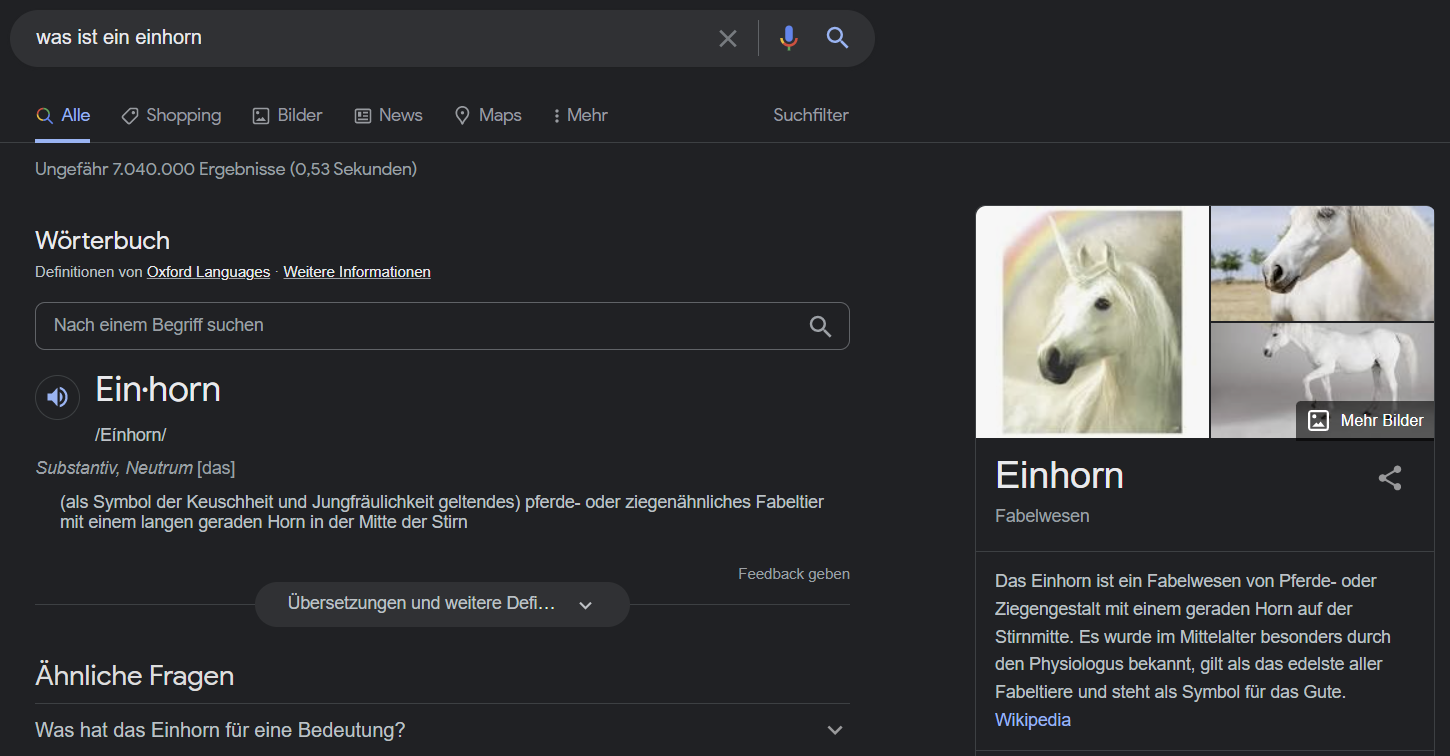
\includegraphics[width=80mm]{images/screenshot_googleQue}
    \caption{Suchergebnis Google}
    \label{fig:screenshotGoogleQue}
\end{figure}
\begin{figure}[ht]
    \centering
    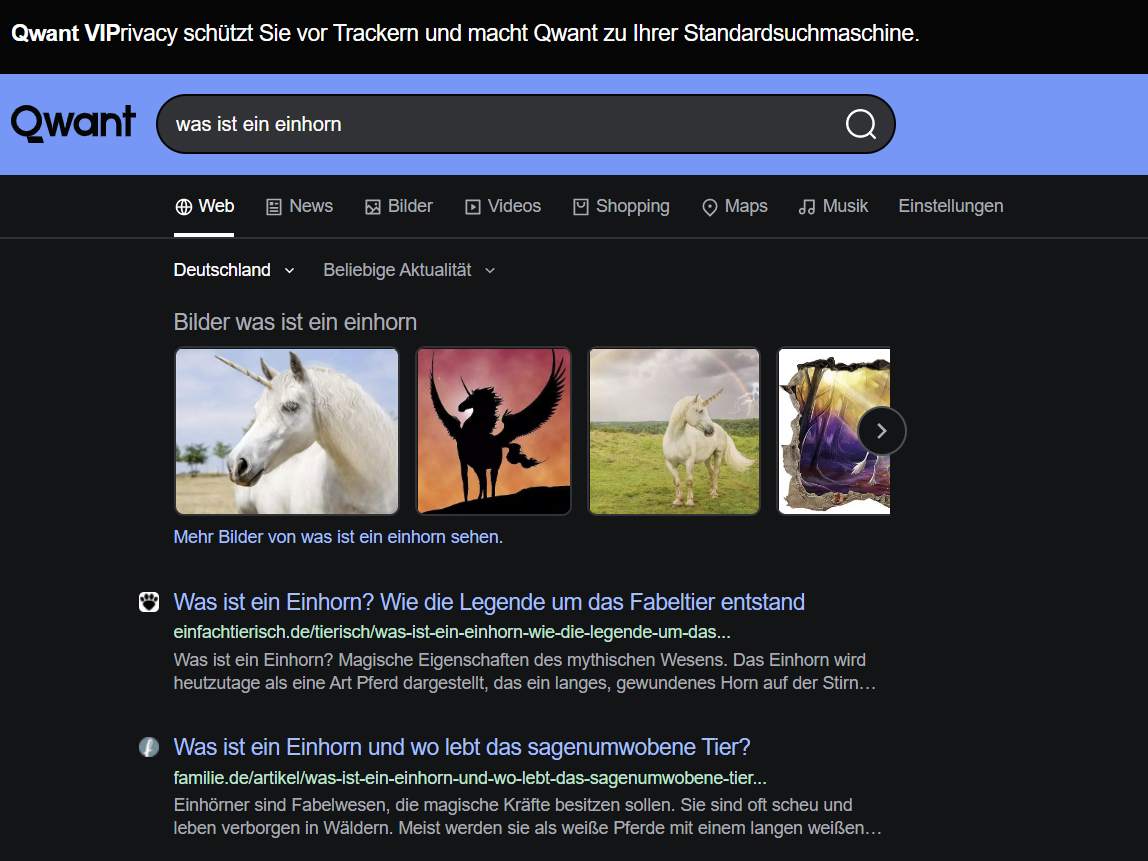
\includegraphics[width=80mm]{images/screenshot_qwantQue}
    \caption{Suchergebnis Qwant}
    \label{fig:screenshotQwantQue}
\end{figure}
Wie man in den angeführten Screenshots sieht, gibt Google direkt die Informationen aus, wo man zum Beispiel bei Qwant zuerst eine Webseite aufrufen muss.
Heute erwarten wir möglichst schnell an die Information zu kommen, worauf sich Google schon angepasst hat.